\chapter{Описание алгоритма}
\section{Предлагаемая схема параллелизации}
Рассмотрим две основные процедуры в алгоритме Фортена с модификацией Буздалова --- $NDHelperA$ и $NDHelperB$.
Обе процедуры являются рекурсивными и следуют принципу <<разделяй и властвуй>>.
Входящие множества точек разделяются на три части $L$, $M$, $H$ относительно медианного значения по $k$-й координате.
Далее $NDHelperA$ и $NDHelperB$, используя тот факт, что точки из подмножества $H$ не могут доминировать точки из $M$, а точки из $M$ не могут доминировать точки из $L$, рекурсивно запускают подзадачи с уменьшением размерности $k$.
Деление задач происходит до того момента, когда размерность $k$ станет равна $2$, что в дальнейшем обрабатывается процедурами $SweepA$ и $SweepB$ соответственно.

\subsection{NDHelperB}
Можно заметить, что на момент вызова процедуры $NDHelperB(L, H, k)$ ранги точек из множества $L$ уже вычислены и в дальнейшем остаются неизменными.
Также заметим, что для корректной работы процедуры, каждая точка из множества $H$ должна быть сравнена с каждой точкой из множество $L$, но при этом порядок сравнений не влияет на результат.

Таким образом мы можем заключить, что рекурсивные вызовы подзадач в теле $NDHelperB$ являются независимыми и порядок их исполнения не влияет на корректность алгоритма.
Более того, мы можем разделить множество $L$ на любое количество частей ${L_1, L_2,\ldots, L_n}$ и тогда результат исполнения $NDHelperB(L_i, H, k)$ для всех $1\leq i\leq n$ будет идентичен результату исполнения $NDHelperB(L, H, k)$.
Следовательно, $NDHelperB$ допускает возможность параллельного исполнения.

\begin{figure}[h]
\centering
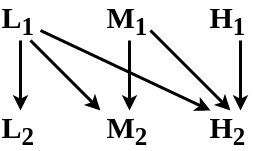
\includegraphics[width=0.4\textwidth]{images/ndb.png}
\caption{Вызовы подзадач в $NDHelperB$}
\label{pic4}
\end{figure}

\subsection{NDHelperA}
С параллелизацией процедуры $NDHelperA$ возникают определенные сложности.
Внутренние вызовы $NDHelperA$ и $NDHelperB$ зависят друг от друга и имеют строго определенную последовательность. 
Например, перед выполнением $NDHelperA(M, k-1)$ вычисления в процедурах $NDHelperA(L, k)$ и $NDHelperB(L, M, k-1)$ уже должны быть выполнены.

Тем не менее, опираясь на утверждение из предыдущей секции, мы можем заметить, что как только ранги какого-то левого подмножества входящих точек будут вычислены, мы сразу же можем начать сравнивать эти точки с подмножествами точек, лежащими правее по $k$-й координате, при помощи процедуры $NDHelperB$.

\begin{figure}[h]
\centering
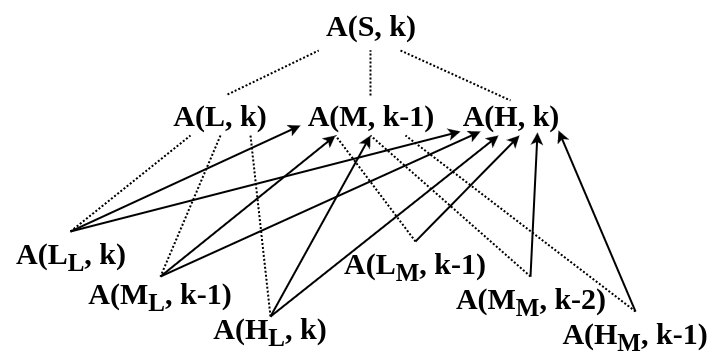
\includegraphics[width=\textwidth]{images/async.png}
\caption{Идея параллелизации процедуры $NDHelperA$}
\end{figure}

Пусть подмножество $L$ в вызове $NDHelperA(L, k)$ посредством $SplitBy$ поделится на три части по $k$-й координате: $L_L$, $M_L$ и $H_L$.
Заметим, что вместо $NDHelperB(L, M, k-1)$ мы можем асинхронно вызывать $NDHelperB(L_L, M, k-1)$, $NDHelperB(M_L, M, k-1)$, $NDHelperB(H_L, M, k-1)$ по мере вычисления рангов каждой из частей.

Аналогичным образом мы можем начать сравнивать точки из $L_L$, $M_L$, $H_L$ и $L_M, M_M, H_M$ с точками из $H$ как только ранги этих точек уже будут известны.
Эту идею можно развить дальше, разделив вызовы $NDHelperB$ на более мелкие подзадачи.

\section{Детали реализации}
Алгоритм был реализован на языке программирования Java с использованием фреймворка Fork/Join, который хорошо подходит для распараллеливания рекурсивных задач.

Все операции перестановок и модификаций осуществляются на массивах индексов, чтобы избежать лишних копирований памяти.
Для нахождения медианного значения заданного критерия по всем точкам используется алгоритм <<Median of medians>> с линейным временем работы.
Операции $split$, $merge$ и поиск медианы изменяют порядок входного массива индексов, поэтому они выполняются на буферах, локальных для каждого потока.
Для поддержания упорядоченных множеств <<ступеней>> Парето-фронтов, описанных в алгоритме Фортена, в $SweepA$ и $SweepB$ используется дерево Фенвика.
По мере выполнения лексикографической сортировки заполняется вспомогательный массив $eqComp$ со следующим свойством: если точка $S_i$ совпадает по каждой координате с точкой $S_j$, то $eqComp[i] = eqComp[j]$, если $S_i$ лексикографически меньше $S_j$, то $eqComp[i] < eqComp[j]$.
Эта структура позволяет в дальнейшем избавиться от лишних сравнений.

$NDHelperB(L, H, k)$ рекурсивно делится на подзадачи в том случае, если $|L|\geq 64$ и $|H|\geq 64$. В противном случае запускается однопоточная версия процедуры.  

\section{Экспериментальное исследование алгоритма}
Ниже будут представлены результаты экспериментального исследования параллельного алгоритма.

В качестве входных данных использовались синтетически сгенерированные массивы случайных величин.
Каждая версия алгоритма запускалась $50$ раз на одной конфигурации размерности и количества точек.
В таблицах указаны минимальное, максимальное и среднее время работы в миллисекундах оригинального алгоритма и параллельной версии на $4$ потоках.
На графиках изображено среднее время исполнения оригинальной версии и параллельной версии на $2$ и $4$ потоках соответственно.

По результатам тестирования можно заключить, что параллельный алгоритм дает заметный прирост в производительности с увеличением $N$ и $M$.
Начиная с $5\cdot 10^4$ точек время работы алгоритма на четырех ядрах сокращается примерно вдвое в сравнении с оригинальной версией.
Тем не менее, на малых размерах входных данных линейный алгоритм показывает более хорошие результаты.
Это связано с накладными расходами, связанными с созданием новых объектов, выделением памяти и копированием контекста.

Тестирование проводилось на компьютере с процессором <<Intel Core i5-3317U>> и 4 гигабайтами оперативной памяти.

\subsection{Сравнение с однопоточной версией алгоритма}
По результатам экспериментов видно, что при больших $N$ достигается неплохой уровень параллелизма.
При $M\leq3$ польза от параллельного исполнения отсутствует, т.к. корневые \textsc{NDHelperB} вызываются с $k=2$, т.е. запускается однопоточная процедура \textsc{SweepB}.

С увеличением $M$ растет количество параллельных подзадач \textsc{NDHelperB}, соответственно прирост в производительности становится более заметным.
Начиная с некоторого значения $M$, глубина дерева исполнения \textsc{NDHelperB} определяется значением $N$ и перестает зависеть от $M$, происходит насыщение всех потоков.

\begin{figure}[h!]
\centering
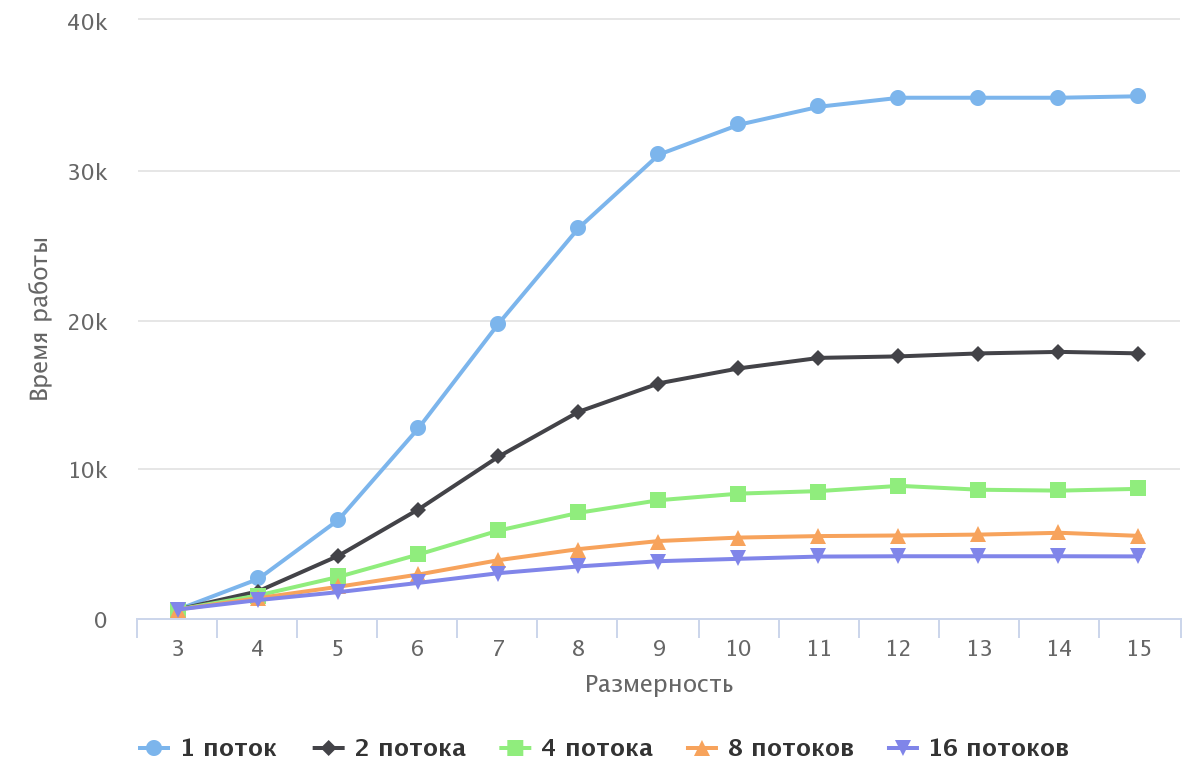
\includegraphics[width=\textwidth]{images/100k.png}
\caption{Медианное время работы\\параллельного алгоритма при $N=10^5$}
\end{figure}

Нам удалось добиться максимального ускорения в $8.47$ раз при $10^5$ точках и 16 потоках.

\begin{table}[h!]
\caption{Время работы алгоритма при $N=10^5$}\label{tab1}
\centering
\begin{tabu}{|*{8}{c|}}
\hline
 & \multicolumn{3}{c|}{Original} & \multicolumn{4}{c|}{Parallel 16 threads}\\
\cline{2-8}
    M & min & max & med & min & max & med & $t_1/t_2$ \\
\hline
    3 & 5.66e+02 & 5.70e+02 & 5.68e+02 & 5.67e+02 & 5.73e+02 & 5.70e+02 & \textbf{1.00}\\ 
    4 & 2.50e+03 & 2.82e+03 & 2.61e+03 & 1.13e+03 & 1.27e+03 & 1.20e+03 & \textbf{2.16}\\
    5 & 6.46e+03 & 6.80e+03 & 6.56e+03 & 1.67e+03 & 1.89e+03 & 1.73e+03 & \textbf{3.79}\\
    6 & 1.26e+04 & 1.28e+04 & 1.27e+04 & 2.28e+03 & 2.45e+03 & 2.35e+03 & \textbf{5.40}\\
    7 & 1.96e+04 & 1.99e+04 & 1.97e+04 & 2.93e+03 & 3.06e+03 & 3.00e+03 & \textbf{6.57}\\
    8 & 2.59e+04 & 2.62e+04 & 2.61e+04 & 3.30e+03 & 3.57e+03 & 3.45e+03 & \textbf{7.57}\\
    9 & 3.08e+04 & 3.12e+04 & 3.10e+04 & 3.69e+03 & 3.91e+03 & 3.80e+03 & \textbf{8.16}\\
    10& 3.28e+04 & 3.32e+04 & 3.30e+04 & 3.85e+03 & 4.03e+03 & 3.96e+03 & \textbf{8.33}\\
    11& 3.41e+04 & 3.45e+04 & 3.42e+04 & 3.99e+03 & 4.24e+03 & 4.11e+03 & \textbf{8.32}\\
    12& 3.46e+04 & 3.51e+04 & 3.48e+04 & 3.98e+03 & 4.25e+03 & 4.13e+03 & \textbf{8.43}\\
    13& 3.46e+04 & 3.51e+04 & 3.48e+04 & 4.00e+03 & 4.36e+03 & 4.13e+03 & \textbf{8.43}\\
    14& 3.46e+04 & 3.50e+04 & 3.48e+04 & 4.01e+03 & 4.43e+03 & 4.13e+03 & \textbf{8.43}\\
    15& 3.47e+04 & 3.52e+04 & 3.49e+04 & 3.95e+03 & 4.25e+03 & 4.12e+03 & \textbf{8.47}\\
\hline
\end{tabu}
\end{table}

\subsection{Сравнение с параллельным алгоритмом Деба}
Для сравнения двух алгоритмов было выбрано относительно небольшое количество точек, т.к. алгоритм Деба из NSGA-II обладает квадратичным временем работы.

По графикам видно, что квадратичный алгоритм лучше масштабируется независимо от $N$. Тем не менее, из-за более плохой асимптотики, он уступает в эффективности предложенному алгоритму при любом количестве потоков от $1$ до $16$. Более того, алгоритм Фортена начинает превосходить шестнадцатипоточный алгоритм Деба уже на четырех потоках.

\begin{table}[h!]
\caption{Сравнение алгоритмов на 16 потоках при $N=10^4$}\label{tab1}
\centering
\begin{tabu}{|*{8}{c|}}
\hline
 & \multicolumn{3}{c|}{Алгоритм Деба} & \multicolumn{4}{c|}{Предложенный алгоритм}\\
\cline{2-8}
    M & min & max & med & min & max & med & $t_1/t_2$ \\
\hline
    3 & 4.80e+02 & 5.03e+02 & 4.91e+02 & 2.69e+01 & 2.72e+01 & 2.70e+01 & \textbf{18.00}\\ 
    4 & 3.29e+02 & 3.83e+02 & 3.53e+02 & 1.16e+02 & 1.41e+02 & 1.34e+02 & \textbf{2.63}\\
    5 & 2.89e+02 & 3.31e+02 & 3.10e+02 & 1.35e+02 & 1.77e+02 & 1.57e+02 & \textbf{1.97}\\
    6 & 2.86e+02 & 3.67e+02 & 3.04e+02 & 1.59e+02 & 2.19e+02 & 1.77e+02 & \textbf{1.72}\\
    7 & 3.07e+02 & 3.89e+02 & 3.23e+02 & 1.65e+02 & 2.19e+02 & 1.86e+02 & \textbf{1.74}\\
    8 & 3.08e+02 & 4.19e+02 & 3.36e+02 & 1.71e+02 & 2.15e+02 & 1.93e+02 & \textbf{1.74}\\
    9 & 3.42e+02 & 3.96e+02 & 3.62e+02 & 1.57e+02 & 2.35e+02 & 1.85e+02 & \textbf{1.96}\\
    10& 3.38e+02 & 4.36e+02 & 3.82e+02 & 1.70e+02 & 2.47e+02 & 1.87e+02 & \textbf{2.04}\\
    11& 3.82e+02 & 5.33e+02 & 4.14e+02 & 1.65e+02 & 2.10e+02 & 1.88e+02 & \textbf{2.20}\\
    12& 3.88e+02 & 4.79e+02 & 4.23e+02 & 1.64e+02 & 2.00e+02 & 1.84e+02 & \textbf{2.30}\\
    13& 4.15e+02 & 4.81e+02 & 4.44e+02 & 1.62e+02 & 2.15e+02 & 1.84e+02 & \textbf{2.41}\\
    14& 4.44e+02 & 5.79e+02 & 4.72e+02 & 1.58e+02 & 2.12e+02 & 1.84e+02 & \textbf{2.57}\\
    15& 4.86e+02 & 5.32e+02 & 5.02e+02 & 1.63e+02 & 2.21e+02 & 1.84e+02 & \textbf{2.73}\\
\hline
\end{tabu}
\end{table}

При большем количестве точек разница в производительности алгоритмов будет прослеживаться более явно из-за разницы в асимптотике и увеличением параллельности нашего алгоритма.

\begin{figure}[h!]
\centering
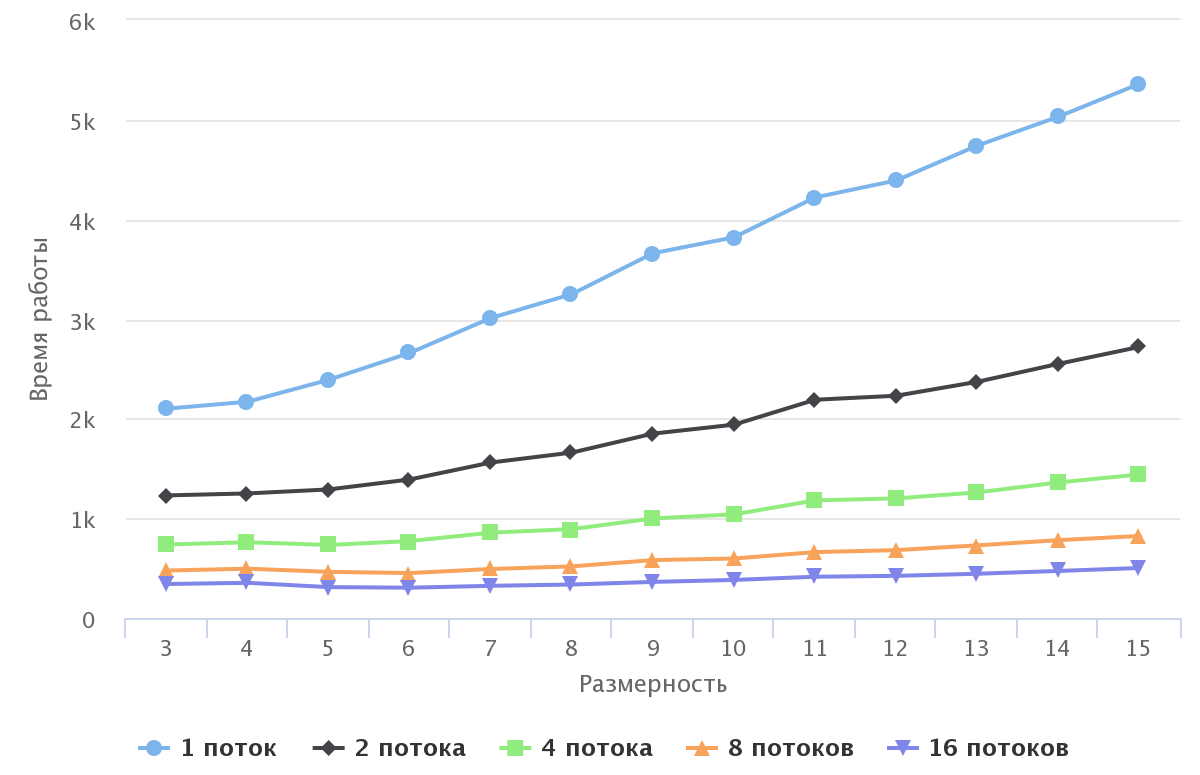
\includegraphics[width=0.95\textwidth]{images/deb10k.png}
\caption{Медианное время работы параллельного алгоритма Деба при $N=10^4$}
\end{figure}

\begin{figure}[h!]
\centering
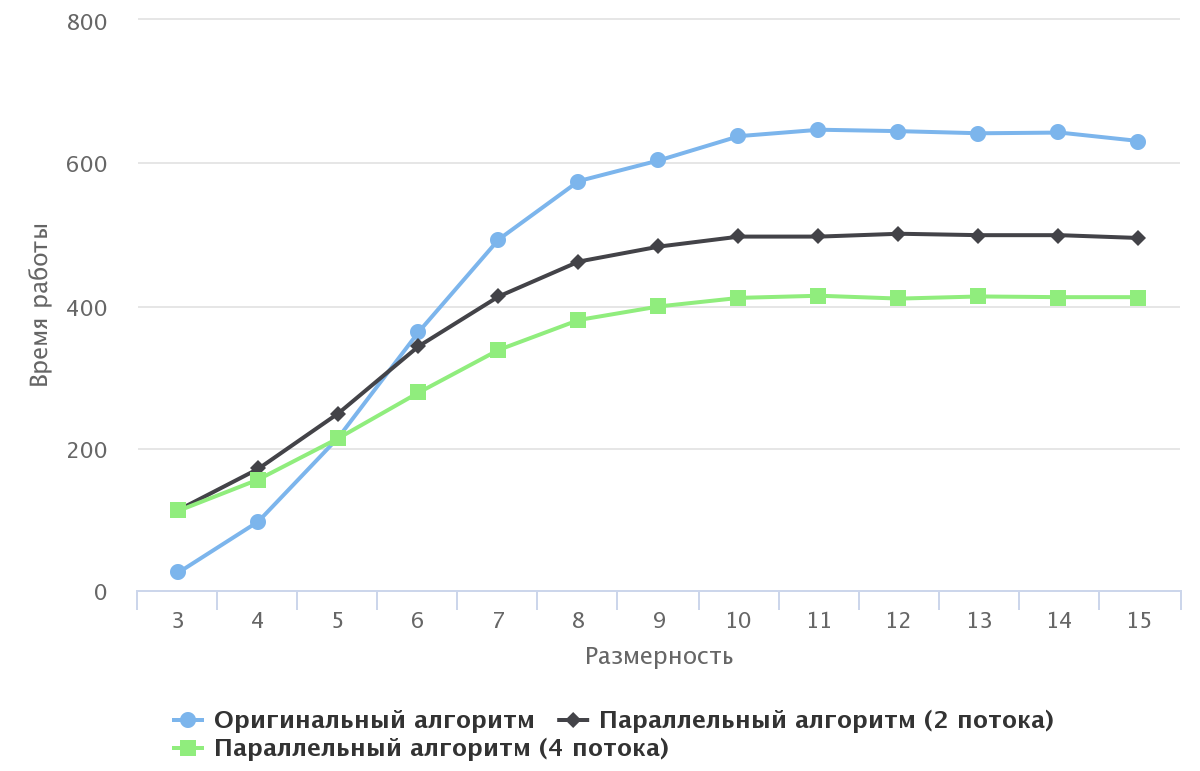
\includegraphics[width=0.95\textwidth]{images/10k.png}
\caption{Медианное время работы параллельного алгоритма Фортена при $N=10^4$}
\end{figure}

